\documentclass[aps,prl,twocolumn,superscriptaddress,reprint,longbibliography,nofootinbib]{revtex4-2}

\usepackage{graphicx}
\usepackage{dcolumn}
\usepackage{bm}
\usepackage[colorlinks,
citecolor=teal,
linkcolor=teal,
urlcolor=teal]{hyperref}
\usepackage{mathrsfs}
\usepackage{amsfonts,amssymb,amsmath,mathtools}
\usepackage{xcolor}
\usepackage{dsfont}
\usepackage{bbm}
\usepackage{physics}
\usepackage{orcidlink}
\usepackage{amsthm}
\usepackage{tikz}
\usepackage[T1]{fontenc}
\newtheorem{theorem}{Theorem}
\newtheorem{conjecture}{Conjecture}

\newcommand{\rev}[1]{\textcolor{red}{#1}}
\newcommand{\trans}{\mathsf{T}}

% === Custom macros ===
\newcommand{\NL}{\mathrm{GNL}}
\newcommand{\RENYI}{\alpha}
\newcommand{\MNL}{\mathrm{M}_2^{\NL}}

\begin{document}

\title{Non-Local Magic Resources for Fermionic Gaussian States}

\author{Daniele Iannotti\orcidlink{0009-0009-0738-5998}}
\email{d.iannotti@ssmeridionale.it}
\thanks{These two authors contributed equally}
\affiliation{Scuola Superiore Meridionale, Largo S. Marcellino 10, 80138 Napoli, Italy}
\affiliation{INFN Sezione di Napoli, via Cintia, 80126 Napoli, Italy}
\affiliation{ Institut für Theoretische Physik, Universität zu Köln, Zülpicher Strasse 77, 50937 Köln, Germany}

\author{Beatrice Magni\orcidlink{0009-0009-8577-0525}}
\email{bmagni@uni-koeln.de}
\thanks{These two authors contributed equally}
\affiliation{ Institut für Theoretische Physik, Universität zu Köln, Zülpicher Strasse 77, 50937 Köln, Germany}

\author{Riccardo Cioli\orcidlink{0009-0001-1286-3773}}
\email{riccardo.cioli3@unibo.it}
\affiliation{Dipartimento di Fisica e Astronomia, Università di Bologna and INFN, Sezione di Bologna, via Irnerio 46, I-40126 Bologna, Italy}

\author{Alioscia Hamma\orcidlink{0000-0003-0662-719X}}
\email{alioscia.hamma@unina.it }
\affiliation{Scuola Superiore Meridionale, Largo S. Marcellino 10, 80138 Napoli, Italy}
\affiliation{Dipartimento di Fisica `Ettore Pancini', Universit\`a degli Studi di Napoli Federico II, Via Cintia, 80126 Napoli, Italy}
\affiliation{INFN Sezione di Napoli, via Cintia, 80126 Napoli, Italy}

\author{Xhek Turkeshi\orcidlink{0000-0003-1093-3771}}
\email{xturkesh@uni-koeln.de}
\affiliation{ Institut für Theoretische Physik, Universität zu Köln, Zülpicher Strasse 77, 50937 Köln, Germany}

\begin{abstract}
Entanglement and magic are fundamental resources that capture the complexity of quantum many-body systems. Non-local magic isolates the irreducible nonstabilizerness intrinsically tied to entanglement. However, evaluating this quantity generally requires a prohibitive minimization over the full Hilbert space, making it computationally inaccessible beyond a few qubits. Here, we overcome this bottleneck by establishing a closed-form expression for the non-local stabilizer entropies of fermionic Gaussian states over local Gaussian unitaries, which we prove at R\'enyi index $\RENYI=2$ for contiguous subsystems of arbitrary size, and which can be evaluated in polynomial time directly from the eigenvalues of the reduced Majorana covariance matrix. We apply this framework to characterize fermionic Gaussian-restricted non-local magic across diverse physical regimes: we derive an exact Page-like curve for typical random states, reveal logarithmic scaling at the quantum critical point of the XY model, and establish a quasiparticle picture for magic generation during out-of-equilibrium quantum quenches. Crucially, because our result relies solely on two-point correlation functions, it provides a scalable route for the experimental estimation of Gaussian-restricted non-local magic in large-scale quantum processors via fermionic shadow tomography.
\end{abstract}
\maketitle
\section{Introduction}

Entanglement and magic, or nonstabilizerness, are two fundamental notions of quantum complexity that capture complementary aspects of what makes a many-body system genuinely quantum~\cite{Horodecki2009,Chitambar2019resources,Veitch2014resource}.
Their operational significance is equally distinct: states with low entanglement admit efficient classical simulation via tensor-network methods~\cite{Schollw_ck_2011}, whereas states with low magic are accessible to stabilizer-based techniques such as tableau simulation~\cite{Gottesman1998,Bravyi2019simulationofquantum} or Pauli propagation~\cite{dowling2025magic,rudolph2025paulipropagationcomputationalframework}.
While entanglement is by now a well-characterized concept in many-body physics~\cite{Laflorencie_2016,amico2008entanglement}, the role of magic has only recently come into focus, driven by the development of stabilizer entropies~\cite{Leone2022SRE,leone2024stabilizer}, scalable probes of nonstabilizerness whose computational cost is comparable to that of entanglement entropy~\cite{huang2026fastexactapproachstabilizer,xiao2026exponentiallyacceleratedsamplingpauli,sierant2026computingquantummagicstate} and which have an important operational meaning~\cite{Bittel_2026, Iannotti_2026, cusumano2025nonstabilizernessviolationschshinequalities}.
This advance has stimulated a broad program of research, from equilibrium phenomena~\cite{piro2,tarabunga2023manybody,oshino2026stabilizer,hoshino2025stabilizerrenyientropyencodes, aditya2025mpembaeffectsquantumcomplexity} to quantum-circuit and Hamiltonian dynamics~\cite{Turkeshi_2025,odavic2025stabilizer,tirrito2025anticoncentration,falcao2025nonstabilizerness, PhysRevB.106.214316, p8dn-glcw, lio2026quantumstatedesignsmagic, aditya2025growthspreadingquantumresources, Viscardi_2026}.

A central open question concerns the interplay between entanglement and magic~\cite{tirrito2024quantifying,szombathy,Iannotti2025entanglement}.
The recently introduced \emph{non-local magic}~\cite{Cao_2025,qian2025quantumnonlocalnonstabilizerness, munizzi2026magicnoncliffordgatestopological, cao2024non} addresses precisely this problem: it isolates the irreducible nonstabilizerness, as quantified by stabilizer entropy, that cannot be removed by local basis changes, thereby separating genuinely correlated magic from purely local contributions.
However, this conceptual advance comes at a steep computational cost: in general, non-local magic is defined through a minimization over all local unitaries acting on the full Hilbert space, rendering it intractable beyond a few qubits. 
Although estimation schemes exist for matrix-product states~\cite{Cao_2025}, where entanglement remains bounded, which broader classes of quantum matter admit an analytic characterization of non-local magic, especially in regimes with extensive entanglement, has remained an open question.

Here, we answer this question for fermionic Gaussian states and unitaries. We introduce the fermionic Gaussian-restricted non-local (GNL) magic.
We prove (cf. Theorem~\ref{thm:global}) that the GNL magic of order $\RENYI=2$ admits a closed-form expression (Eq.~\eqref{eq:analytic_NL}) in terms of the eigenvalues of the reduced Majorana covariance matrix on a contiguous subsystem of size $\ell$, computable with $\mathrm{poly}(\ell)$ resources. 
The key insight behind this result is that the minimization over local \emph{Gaussian} unitaries is solved exactly by the BCS canonical form~\cite{BoteroReznik2004}. 
This is in stark contrast with the total magic, which requires Majorana Monte Carlo~\cite{Bera_2025} or perfect sampling~\cite{collura2026nonstabilizernessfermionicgaussianstates}, both converging in general with an exponential number of samples.
We leverage this result to obtain a series of rigorous physical insights: an exact Page-like curve for typical fermionic Gaussian states, corroborated numerically by SYK$_2$ eigenstates~\cite{Bera_2025,santra2025complexitytransitionschaoticquantum,jasser2025stabilizer, malvimat2026multipartitenonlocalmagicsyk, njgn-fksh}; logarithmic scaling of non-local magic at the XY critical point, captured analytically via the Fisher--Hartwig approach; a quasiparticle picture~\cite{calabrese2009} for magic spreading after quantum quenches; and diffusive growth in brickwork Gaussian random circuits.
Because our result relies solely on two-point correlation functions, it also provides a scalable route for the experimental estimation of Gaussian-restricted non-local magic in large-scale quantum processors via fermionic shadow tomography~\cite{Wan_2023}.

\section{Methods}

We begin by introducing the notation and key definitions; we refer to Refs.~\cite{Mbeng2024,surace,sierant2026fermionic,sierant2026theorymatchgatecommutant} for pedagogical introductions.
We consider fermionic Gaussian systems on $N$ qubits in a lattice $\Lambda=\{1,\dots, N\}$, described by a Hilbert space of dimension $d=2^N$.
The natural degrees of freedom are the $2N$ Majorana operators $\gamma_j$, obtained via the Jordan--Wigner transformation $\gamma_{2j-1} = \bigl(\prod_{m=1}^{j-1} Z_m\bigr)X_j$ and $\gamma_{2j} = \bigl(\prod_{m=1}^{j-1} Z_m\bigr)Y_j$, where $X_j$, $Y_j$, $Z_j$ are the Pauli operators on qubit $j$.
These operators are Hermitian, $\gamma_j=\gamma_j^\dagger$, and satisfy the Clifford algebra $\lbrace \gamma_j,\gamma_k\}=2 \delta_{jk} \mathbb{I}$.

Fermionic Gaussian unitaries (FGU), or matchgates, are the operators that act adjointly on Majorana as rotations $U_O\gamma_j U_O^\dagger = \sum_{m}O_{mj}\gamma_m$, with $O\in \mathrm{O}(2N)$; they form a group, which we denote $\mathfrak{M}_N$. 
Orthogonal matrices can be decomposed as $O=R^{(1-\det O)/2}Q$ with $Q\in \mathrm{SO}(2N)$ and $R=\mathrm{diag}(1,-1,\dots,-1)$  a reflection.
This implies that $U_O=X_1^{(1-\det(O))/2}\exp[-iH]$ is split into a part induced by special orthogonal transformations, captured by the so-called fermionic Gaussian Hamiltonians 
\begin{equation}
    H= \frac{i}{4}\sum_{m,n=1}^{2N} h_{m,n} \gamma_m\gamma_n\;,\label{eq:ham}
\end{equation}
where $h=-h^T$ is the $2N\times 2N$ antisymmetric matrix such that $Q=\exp[h]$, and the implementation of the reflection $R$ via the Pauli operator $X_1=\gamma_1$. 

A pure fermionic Gaussian state (FGS), or free fermionic state, is defined by $|\Psi_O\rangle=U_O|\mathbf{0}\rangle$ for the fermionic Gaussian unitary induced by $O\in \mathrm{O}(2N)$, and $|\mathbf{0}\rangle\langle\mathbf{0}| = d^{-1}\prod_{m=1}^{N}(\mathbb{I}-i\gamma_{2m-1}\gamma_{2m})$ is the fermionic vacuum state. 
Denoting for any pure state $|\Psi\rangle$ the covariance matrix $\Gamma_{mn}=i\langle \Psi|[\gamma_m,\gamma_n]|\Psi\rangle/2$, fermionic Gaussian states are fully characterized by the covariance matrix. In fact, given the vacuum covariance matrix
\begin{equation}
    \Gamma_0= { \bigoplus_{m=1}^N \begin{pmatrix}
        0 &-1 \\1&0
    \end{pmatrix}}\;,
\end{equation}
using the adjoint transformation, one obtains that $|\Psi_O\rangle\langle \Psi_O|$ is uniquely fixed by $\Gamma= O\Gamma_0 O^T$. 
For pure fermionic Gaussian states and any bipartition $\Lambda=A\sqcup B$ with $|A|=\ell\le N/2$ (made precise below), Ref.~\cite{BoteroReznik2004} showed that local Gaussian transformations $O_A\oplus O_B$ of the Majorana modes are sufficient to bring the state into a canonical modewise form of independent two-mode BCS-like pairs 
\begin{equation}
\begin{split}
     |\Psi_{\mathrm{can}}\rangle
:= (T_{\sigma_{A}}\otimes T_{\sigma_{B}})\bigotimes_{i=1}^{\ell} [|\mathrm{B}(\theta_i)\rangle]\otimes |0\rangle^{\otimes (N-2\ell)}\;,
\end{split}
\label{eq:can_form}
\end{equation} 
where $|\mathrm{B}(\theta_i)\rangle=\cos\theta_i\,|00\rangle_i+\sin\theta_i\,|11\rangle_i$  and $T_{\sigma_X}$ are permutations that act separately on qubits in $X\in \{A,B\}$. This form is analogous to the Schmidt decomposition for pure fermionic Gaussian states, and it is fundamental for the main result.

\subsection{Non-local magic and its fermionic counterpart}

We now present our main quantity: non-local magic.
We recall that the stabilizer entropy of order $\RENYI$ is defined for a pure state $|\Psi\rangle$ as $M_\RENYI(|\Psi\rangle)=(1-\RENYI)^{-1}\log_2 \zeta_\RENYI(|\Psi\rangle)$~\cite{Leone2022SRE}, where $\zeta_\RENYI= d^{-1}\sum_{P\in \mathcal{P}_N} \langle \Psi|P|\Psi\rangle^{2\RENYI}$ is the stabilizer purity and $\mathcal{P}_N=\{ \mathbb{I},X,Y,Z\}^{\otimes N}$  is the set of $N$-qubit Pauli strings. This quantity is a magic monotone for integer $\RENYI\ge 2$~\cite{piro,leone2024stabilizer}.

Throughout this work, we consider the bipartition $\Lambda = A\sqcup B$ of the chain into the contiguous blocks $A=\{1,\dots,\ell\}$ and $B=\{\ell+1,\dots,N\}$. The non-local magic (NLM) of a pure state is defined as 
\begin{equation}
    M_\RENYI^\textup{NL}:= \min_{U_A , U_B} M_\RENYI\left[(U_A\otimes U_B)|\Psi\rangle\right]\;,\label{eq:defNLmagic}
\end{equation}
where the minimization is over $\mathrm{U}(d_A)\otimes \mathrm{U}(d_B)$ with $d_A=2^{\ell}$ and $d_B = 2^{N-\ell}$. This is the magic that cannot be erased or extracted by local unitary operations. This notion is cognate to (but distinct from) that of {\em long-range magic}, that is, the non-stabilizerness that cannot be removed by finite-depth local unitary circuits \cite{Korbany2025}. One salient distinction is that maximally entangled states have vanishing non-local magic as they are locally equivalent to stabilizer states.
This minimization is superexponentially costly, rendering non-local magic intractable beyond a handful of qubits.
In Ref.~\cite{Cao_2025}, it was shown that for $\RENYI = 2$ a reliable proxy for non-local magic can be obtained from the Schmidt spectrum of the state over the same bipartition.


To study fermionic Gaussian states and their non-local magic, we introduce the fermionic Gaussian-restricted non-local magic
\begin{equation}
    M_\RENYI^\textup{GNL}:= \!\!\min_{U_{O_A} , U_{O_B}} \!\!M_\RENYI\left[(U_{O_A}\otimes U_{O_B})|\Psi\rangle\right],\label{eq:defGNLmagic}
\end{equation}
where now the minimization is over the Gaussian unitaries induced by $\mathrm{O}(2\ell)\oplus \mathrm{O}(2(N-\ell))$, hence $ M_\RENYI^\textup{NL} \leq  M_\RENYI^\textup{GNL}$. Since $A$ and $B$ are contiguous blocks of the Jordan--Wigner chain, $U_{O_A}\otimes U_{O_B}$ is itself a Gaussian unitary of the whole chain, induced by $\mathrm{O}(2\ell)\oplus\mathrm{O}(2(N-\ell))$ (see Appendix~\ref{app:proof:dpp}).
Throughout this work our main interest is the case $\RENYI=2$, the smallest R\'enyi index for which the stabilizer entropy is a magic monotone~\cite{piro,leone2024stabilizer}, the most studied in the literature, and the one we implicitly refer to when writing simply \emph{Gaussian-restricted non-local magic}. Nevertheless, we will also comment on results for $\RENYI>2$, in particular in Appendix~\ref{Sec:generaliz}.
Our main result is that, for fermionic Gaussian states, the Gaussian-restricted non-local magic can be evaluated exactly in $\mathrm{poly}(N)$ resources.

\section{Results}

Consider a pure fermionic Gaussian state $|\Psi_O\rangle$ with covariance matrix $\Gamma=O \Gamma_0 O^T$ and the bipartition $\Lambda = A\sqcup B$ into the contiguous blocks $A=\{1,\dots,\ell\}$ and $B=\{\ell+1,\dots,N\}$. 
Our main result shows that the GNL magic is entirely determined by the spectrum of the reduced covariance matrix. Let $\{\lambda_i\}_{i=1,\dots,\ell}$ denote the non-negative eigenvalues of the $2\ell\times 2\ell$ reduced covariance matrix $i\Gamma_A := i\Gamma|_{\mathcal{I}_A}$ of the Majorana modes restricted to $A$, $\mathcal{I}_A:=\{2m-1,2m\;|\; m\in A\}$. Then, our main finding is the following closed-form expression at $\RENYI=2$.

\begin{theorem}[Gaussian-restricted non-local magic of Gaussian states at $\RENYI=2$]
\label{thm:global}
Let $|\Psi_O\rangle$ be an arbitrary pure fermionic Gaussian state on $N$ modes and let $\Lambda=A\sqcup B$ be the bipartition into the contiguous blocks $A=\{1,\dots,\ell\}$ and $B=\{\ell+1,\dots,N\}$. Then
\begin{equation}
\begin{split}
    M_{2}^{\mathrm{GNL}}(|\Psi_O\rangle)&=\sum_{i=1}^{\ell}\mathfrak{m}_2(\lambda_i^2)\;,\\
    \mathfrak{m}_2(x)&=-\log_2\!\left(1-x+x^2\right),
\end{split}
    \label{eq:analytic_NL}
\end{equation}
or, equivalently, in terms of the stabilizer purity,
\begin{equation}
\begin{split}
\max_{\substack{O_A\in \mathrm{O}(2\ell)\\ O_B\in \mathrm{O}(2(N-\ell))}}\!\!\!\!\zeta_2&\left[(U_{O_A}\otimes U_{O_B})|\Psi_O\rangle\right]\\ &=\prod_{i=1}^{\ell}\left(1-\lambda_i^2+\lambda_i^4\right)\;,
\end{split}
\label{eq:thm_zeta}
\end{equation}
the maximum being attained in the Botero--BCS canonical axes of Eq.~\eqref{eq:can_form}.
\end{theorem}

The proof is given in full detail in Appendix~\ref{app:proof}. It assumes that the state $|\Psi_O\rangle$ is pure and Gaussian, and uses that $A$ and $B$ are contiguous blocks, which guarantees that Eq.~\eqref{eq:defGNLmagic} amounts to a maximization of the stabilizer purity over the orbit of the covariance matrix under $O_A\oplus O_B$.
The key point is that local Gaussian unitaries over a bipartition of the system bring any pure fermionic Gaussian state into a canonical modewise form $\ket{\Psi_{\rm can}}$ in Eq.~\eqref{eq:can_form}, consisting of independent two-mode Bell-like pairs~\cite{BoteroReznik2004}, a normal form that underlies several equivalent descriptions of fermionic Gaussian entanglement~\cite{SpeeSchwaigerGiedkeKraus2018,MorralYepesLangerGammonSmithKrausPollmann2025,langer2026matchgatecircuitrepresentationfermionic}.
We prove that this representative is the \emph{global} maximizer of the stabilizer purity $\zeta_2$ on the local Gaussian orbit, i.e.
$M_{2}^{\mathrm{GNL}}(|\Psi_O\rangle) = M_{2}(|\Psi_{\rm can}\rangle)$,
from which Eq.~\eqref{eq:analytic_NL} follows by direct computation of the two-mode stabilizer entropy~\cite{Cao_2025,qian2025quantumnonlocalnonstabilizerness}.


For integer $\RENYI>2$ we conjecture that the same structure survives, with the R\'enyi weight adapted accordingly,
    \begin{equation} 
    \begin{split}
      M_{\RENYI}^{\mathrm{GNL}}(|\Psi_O\rangle)\! &= \sum_{i=1}^{\ell}\mathfrak{m}_\RENYI(\lambda_i^2)\;,
    \end{split}
    \label{eq:analytic_NL_alpha}
    \end{equation}
\noindent
where $\mathfrak{m}_\RENYI(x)$ is the weight function
\begin{equation}
    \begin{split}
      \mathfrak{m}_\RENYI(x)&:=
    \frac{1}{1-\RENYI}\log_2\! \left[\frac{\left(1-x \right)^{\RENYI }\!\!+1+ x^{ \RENYI }}{2} \right]\;, 
    \end{split}
    \label{eq:analytic_NL_weights}
    \end{equation}
which reduces to Eq.~\eqref{eq:analytic_NL} at $\RENYI=2$. This conjecture is supported by the extensive variational optimization reported in Appendix~\ref{app:variational}, and it reproduces the same phenomenology as the $\RENYI=2$ case, as we discuss in Appendix~\ref{Sec:generaliz}.

Several remarks are in order.
First, the proof of Theorem~\ref{thm:global} relies heavily on the specific quadratic (collision) functional form. Proving the result for $\RENYI>2$ would require a different proof strategy, which we leave open for future investigations.
Second, for small subsystems the restriction to Gaussian unitaries is immaterial. For $\ell\le 2$, structural simplifications make the Gaussian minimization coincide with the full one, $M_2^{\mathrm{NL}}=M_2^{\mathrm{GNL}}$, and Eq.~\eqref{eq:analytic_NL} reproduces the expression obtained in Ref.~\cite{Cao_2025} from the Schmidt spectrum. For larger subsystems, this is no longer the case: non-Gaussian local transformations can further decrease the magic even when the initial state is Gaussian, so that Theorem~\ref{thm:global} provides an upper bound on the generic non-local magic, $M_2^{\mathrm{NL}}\le M_2^{\mathrm{GNL}}$.
Lastly, our formula is considerably simpler even than computing the \emph{total} stabilizer entropy $M_\RENYI$ for fermionic Gaussian states, which requires either Majorana Monte Carlo~\cite{Bera_2025} or perfect sampling~\cite{collura2026nonstabilizernessfermionicgaussianstates}, both requiring an exponential number of samples for convergence in the worst case. In contrast, evaluating $M_\RENYI^\mathrm{GNL}$ via Eqs.~\eqref{eq:analytic_NL} and~\eqref{eq:analytic_NL_alpha} requires only $\mathrm{poly}(\ell)$ operations.

In the following, we will consider throughout the case $\RENYI=2$, where the stabilizer entropy is a magic monotone and where Theorem~\ref{thm:global} applies. (Nevertheless, as aforementioned, we have checked that the same phenomenology holds for $\RENYI>2$, see Appendix~\ref{Sec:generaliz}.)
We will show that the structure highlighted in Eq.~\eqref{eq:analytic_NL} enables several analytical results, both at equilibrium and out-of-equilibrium.

\subsection{Typical Gaussian states}

Having established the exact formula, we first investigate the Gaussian-restricted non-local magic of \emph{typical} Gaussian states, i.e., states $|\Psi_O\rangle=U_O|\mathbf{0}\rangle$ generated by Haar-random $O\in \mathrm{O}(2N)$.
Our goal is to compute the average $\overline{M}_2^\mathrm{GNL}\equiv \mathbb{E}_{O\sim \mathrm{O}(2N)}[M_2^\mathrm{GNL}(|\Psi_O\rangle)]$, which for our closed-form expression reduces to a random matrix theory problem~\cite{Mehta2004,Livan_2018,vidmar2017entanglement}.

For a fixed subsystem $A$ of size $\ell\le N/2$, let us define the stochastic variables $x_k:=\lambda_k^2$, whose joint probability distribution is a Jacobi ensemble~\cite{Mehta2004,PhysRevB.103.L241118}

We emphasize that this is a \emph{quenched} average --- performed outside the logarithm --- which is typically harder to evaluate than its annealed counterpart.

\begin{figure}[t!]
    \centering
    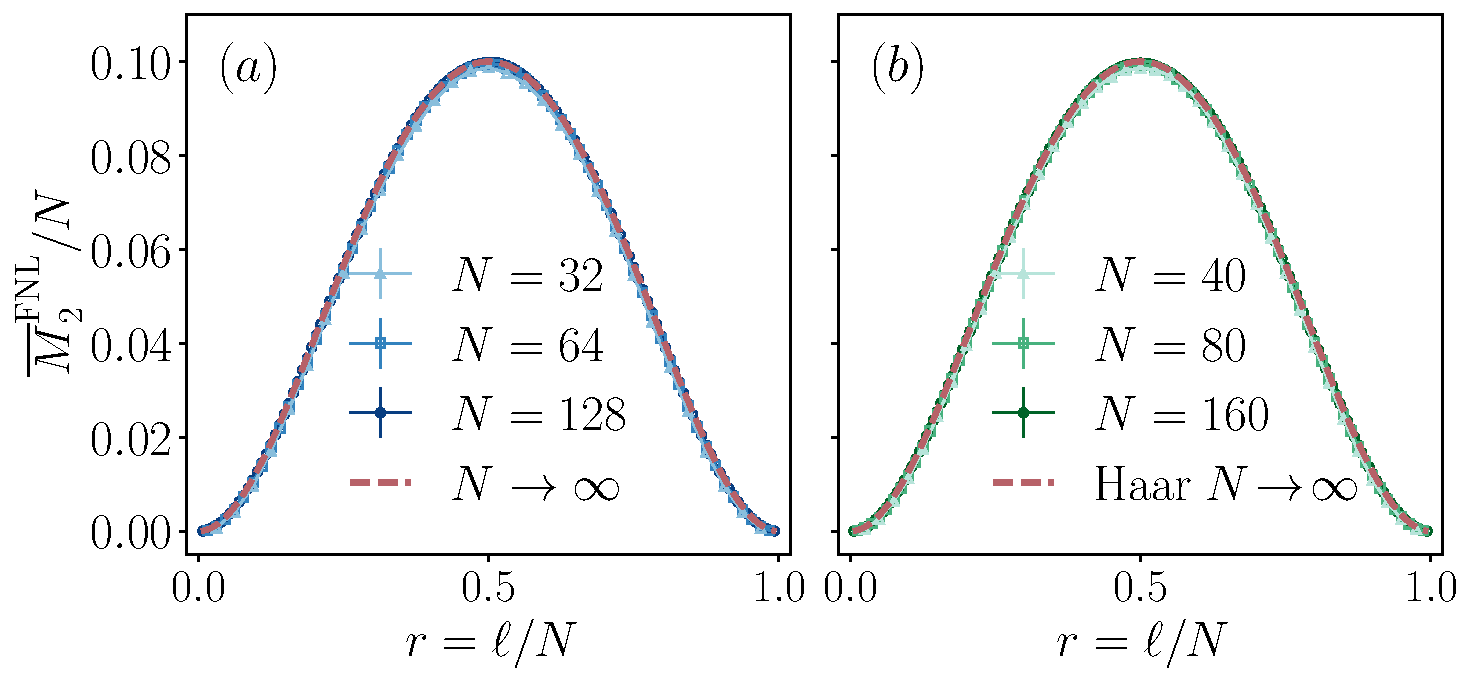
\includegraphics[width=\columnwidth]{../fig1_typicality.pdf}
    \caption{\textbf{Gaussian-restricted non-local magic of typical fermionic Gaussian states.}
    (a)~Page curve for Haar-random FGS: $\overline{M_2}^{\mathrm{GNL}}/N$ is plotted against the ratio $r=\ell/N$. The results are compared with the closed form expression for $N\to\infty$ in Eq.~\eqref{eq:ziopin2}.
    (b)~The Gaussian-restricted non-local magic Page curve is tested against the numerically computed average non-local magic for SYK$_2$ mid-spectrum eigenstates. The results are in quantitative agreement with Eq.~\eqref{eq:ziopin2}. }
    \label{fig:typicality}
\end{figure}

We now turn to the thermodynamic limit $\ell,N\to\infty$ at fixed ratio $r=\ell/N\in[0,1/2]$, defining the Gaussian-restricted non-local magic density $\overline{\mathsf{m}}_2^\mathrm{GNL}:=\overline{M}_2^\mathrm{GNL}/N$ (the final result is symmetric under $r\to 1-r$).

\begin{equation}
\overline{\mathsf{m}}_2^\mathrm{GNL}(r)\simeq \frac{c}{\pi}\int_0^{\pi/2} \frac{\cos^2 \theta}{1-c\sin^2\theta} \mathfrak{m}_2(c\sin^2 \theta)d\theta\;.\label{eq:ziopin2}
\end{equation}
At exactly half bipartition, $r=1/2$, this integral can be performed exactly and the formula reduces to 
$\overline{\mathsf{m}}_2^\mathrm{GNL}(r)\simeq 2-\log_2(2+\sqrt{3})$.
On the other hand, for small $r\simeq 0$ (and by symmetry $r\simeq 1$), we have $c\simeq 4r$ and the integral yields $\overline{\mathsf{m}}_2^\mathrm{GNL}(r\simeq 0)\simeq \frac{r^2}{\ln(2)}+\mathcal{O}(r^3)$. 
This {\em Gaussian-restricted non-local magic Page curve} shows a  quadratic onset,  for every $\RENYI$ (see Appendix Sec.~\ref{Sec:generaliz}), with a transparent physical origin: when $\ell$ is of order one while $N\to\infty$, the $\ell$ modes of $A$ are almost, or exactly, maximally entangled and thus carry no non-local magic. 
This is in sharp contrast with the entanglement Page curve, which vanishes only at $|A|=0$ and grows linearly for small $r$~\cite{PhysRevE.106.034118,PhysRevLett.125.180604,PhysRevB.103.L241118}.

To test the universality of this result beyond Haar-random states, we consider the Sachdev--Ye--Kitaev model at quadratic order, $\mathrm{SYK}_2$.

In Fig.~\ref{fig:typicality}(b), we plot the resulting non-local magic density $\overline{\mathsf{m}}_2^\mathrm{GNL}$ versus $r=\ell/N$ for $N=40,80,160$.
The data converge to the analytical Haar prediction Eq.~\eqref{eq:ziopin2} as $N$ increases, confirming that mid-spectrum eigenstates of SYK$_2$ reproduce the typicality of Gaussian-restricted non-local magic expected from random fermionic Gaussian states.

\subsection{Ground states of XY model}

\begin{figure*}
    \centering
    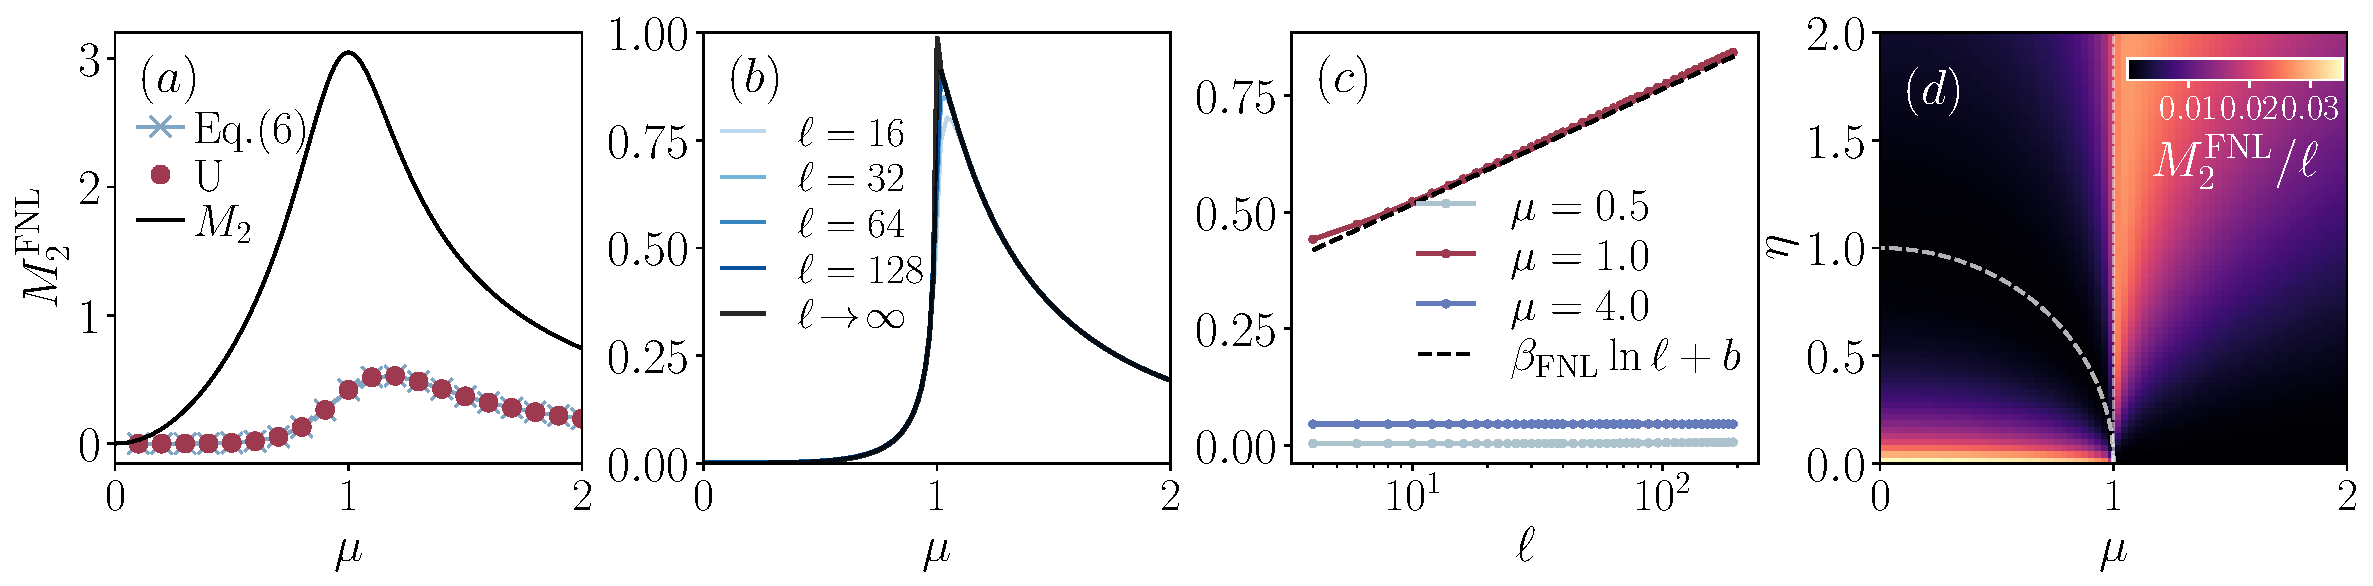
\includegraphics[width=\linewidth]{../fig1_equilibrium.pdf}
    \caption{%
    \textbf{Equilibrium Gaussian-restricted non-local magic in the Ising and XY models.}
    (a)~Validation of Eq.~\eqref{eq:analytic_NL} for the Ising ground state with $N=8$, $\ell=4$: the Gaussian-restricted non-local magic $M_2^{\mathrm{GNL}}$ from Eq.~\eqref{eq:analytic_NL} (crosses) agrees with the brute-force minimization over all local unitaries $U_A \otimes U_B$  (red marker) to numerical precision. The black line shows the total stabilizer entropy $M_2$ for reference.
    (b)~$M_2^{\mathrm{GNL}}$ vs.\ transverse field $\mu$ in the thermodynamic limit for subsystem sizes $\ell = 16, 32, 64, 128$; the black curve is the exact $\ell \to \infty$ result from the Peschel entanglement spectrum, Eq.~\eqref{eq:NL_peschel2}. The Gaussian-restricted non-local magic peaks at the critical point $\mu_c = 1$ and is suppressed in both gapped phases.
    (c)~Scaling of $M_2^{\mathrm{GNL}}(\ell)$ at criticality ($\mu = 1$, red): logarithmic growth: the dashed line is the fit $\beta_{\mathrm{fit}}\ln\ell+b$,  with $\beta_{\mathrm{fit}} \approx 0.1072$  and $b \approx 0.27$, in agreement with the Fisher--Hartwig prediction Eq.~\eqref{eq:alpha_NL}. In the gapped phases ($\mu = 0.5$, $\mu = 4.0$), $M_2^{\mathrm{GNL}}$ saturates to a finite value.
    (d)~Heatmap of $M_2^{\mathrm{GNL}}/\ell$ over the XY phase diagram ($\mu$, $\eta$), computed from the exact Peschel formula. The Gaussian-restricted non-local magic is concentrated near the critical lines and is strongly suppressed deep in the gapped phases.
    }
    \label{fig:Ising_model}
\end{figure*}

We now apply Eq.~\eqref{eq:analytic_NL} to study the equilibrium properties of Gaussian-restricted non-local magic in the ground state of the XY chain
\begin{equation}
    H = -\sum_{j=1}^{N}\!\left[\frac{1+\eta}{2}X_j X_{j+1} + \frac{1-\eta}{2}Y_j Y_{j+1} + \mu Z_j\right],
    \label{eq:xy}
\end{equation}
with periodic boundary conditions.

Throughout this Section, the XY chain is studied as a \emph{fermionic} model, i.e.\ as a Majorana chain: after the Jordan--Wigner mapping the ground state is naturally written --- and exactly solvable --- as a fermionic Gaussian state, and the natural notion of locality is that of the fermionic modes. 
Accordingly, $M_\RENYI^{\mathrm{GNL}}$ is the non-local magic of the \textit{free-fermion problem}, and the local Gaussian unitaries of Eq.~\eqref{eq:defGNLmagic} are, for a contiguous cut, implemented by genuine tensor products $U_{O_A}\otimes U_{O_B}$ of qubit unitaries (cf. also Appendix~\ref{app:proof}).
Following standard practice in the literature, we simplify the nomenclature and keep referring to it as the XY model~\footnote{Note that, minimizing over all local spin unitaries would give a quantity bounded from above by ours, $M_\RENYI^{\mathrm{NL}}\le M_\RENYI^{\mathrm{GNL}}$, as discussed in the first remark below Theorem~\ref{thm:global}.}. 

From now on, we consider the bipartition fixed by the contiguous interval $A=\{1,\dots,\ell\}$ and its complement $B=\Lambda\setminus A$.
In the thermodynamic limit $N\to\infty$ with $\ell$ fixed, the reduced covariance matrix $\Gamma_A$ is a $2\ell\times 2\ell$ block-Toeplitz matrix with $2\times 2$ blocks depending only on $m-n$,

The Gaussian-restricted non-local magic $M_2^{\mathrm{GNL}} = \sum_n \mathfrak{m}_2(\lambda_n^2)$ is therefore a spectral function of $\Gamma_A$ with symbol $g(k)$, providing a direct route to efficient numerical evaluation.
For a given Hamiltonian and subsystem size $\ell$, we construct $\Gamma_A$ by evaluating the integral in Eq.~\eqref{eq:block_toeplitz}, exact in the thermodynamic limit $N\to\infty$, and compute the non-local magic via Eq.~\eqref{eq:analytic_NL} from the eigenvalues $\pm\lambda_n$ ($\lambda_n\in[0,1]$) of $i\Gamma_A$.
This procedure reaches large subsystem sizes $\ell$ at classical computational cost $\mathcal{O}(\ell^3)$.

In the scaling limit $N\gg \ell\gg 1$, the asymptotic behavior of spectral functions of Toeplitz matrices is controlled by two classical results: the \emph{strong Szeg\H{o} theorem}, applicable when the symbol is smooth, and the \emph{Fisher--Hartwig formula}, which governs the corrections arising from singularities in the symbol~\cite{Jin_2004,Its_2005}.

Since the symbol~\eqref{eq:block_toeplitz} satisfies $|\det g(k)| = 1$ for all $k$, the Szeg\H{o} theorem rules out volume-law scaling of $M_2^{\mathrm{GNL}}$.
When $g(k)$ is smooth, as occurs in the gapped phases $\mu \neq 1$ where $\theta_k$ is analytic, the strong Szeg\H{o} theorem further implies that $M_2^{\mathrm{GNL}}$ saturates to a finite value as $\ell \to \infty$, with exponentially small corrections~\cite{simon2010szego}.
Logarithmic growth can arise only from singularities in the symbol, which for the Ising model ($\eta=1$) occur at the critical point $\mu = \mu_c = 1$, where the Bogoliubov angle $\theta_k$ develops a jump discontinuity at $k = 0$.
We now exploit this structure to obtain exact scaling forms in both regimes.

\subsubsection{Exact results off criticality via corner transfer matrices}

For the XY model away from criticality, the entanglement spectrum of a semi-infinite bipartition fixed by $A=\mathbb{Z}_+=\{1,2,\dots\}$ is known in closed form through the corner transfer matrix approach~\cite{Peschel2009,Eisler2017}.
As we show below, this leads to the exact computation of $M_2^\mathrm{GNL,\mathbb{Z}_+}$ in this regime. 
This regime approximates the scaling limit $N\gg\ell\gg1$.
The single-particle entanglement energies are equally spaced,
\begin{equation}
    \varepsilon_n^{\mathrm{ent}} = \begin{cases}
        (2n+1)\,\varepsilon & \mu > 1 \;,\\
        2n\,\varepsilon & \mu < 1 \;,
    \end{cases}
    \label{eq:peschel_spectrum}
\end{equation}

For a block of $\ell$ sites in the infinite chain with periodic boundary conditions, two separate boundaries contribute, so that the Gaussian-restricted non-local magic is twice the single-cut result
\begin{equation}
    M_2^{\mathrm{GNL}}(\ell) \simeq  2M_2^{\mathrm{GNL},\mathbb{Z}_+} = 2\sum_{n=0}^{\infty} \mathfrak{m}_2\!\left[\tanh^2\left(\frac{\varepsilon_n^{\mathrm{ent}}}{2}\right)\right],
    \label{eq:NL_peschel2}
\end{equation}
up to corrections exponentially small in $\ell/\xi$, where $\xi$ is the correlation length of the problem. 
Since $\mathfrak{m}_2(x)\simeq(1-x)/\ln 2$ vanishes linearly as $x \to 1$, and $1-\lambda_n^2 \to 0$ exponentially for large $n$, the series converges rapidly: for $\mu$ away from criticality, only a few terms contribute, consistently with the Szeg\H{o} prediction of a finite $M_2^{\mathrm{GNL}}$.

In Fig.~\ref{fig:Ising_model} we benchmark these predictions against numerical simulations with periodic boundary conditions for the Ising model ($\eta=1$).
In Fig.~\ref{fig:Ising_model}(a), we validate Eq.~\eqref{eq:analytic_NL} by comparing against a brute-force minimization over the full unitary group $\mathrm{U}(d_A)\otimes\mathrm{U}(d_B)$ for $N=8$, $\ell=4$: the two results agree to numerical precision. For a general model (i.e., beyond Ising or XY), however, we do not expect such agreement, and only the inequality
$M_2^{\mathrm{NL}}\le M_2^{\mathrm{GNL}}$ is expected to hold,
cf.~Appendix~\ref{app:variational}~\footnote{We nevertheless find that throughout the XY phase
diagram, for the system sizes accessible to exact minimization, the agreement persists, see Ref.~\cite{zenodo}.}.

In Fig.~\ref{fig:Ising_model}(b), we compare exact numerics for $N=10^6$ qubits and $\ell = 16,32,64,128$ with the asymptotic formula Eq.~\eqref{eq:NL_peschel2}, finding quantitative agreement.

At the critical point $\mu_c=1$ ($\eta=1$), the gap closes and the correlation length diverges as $\xi\simeq |\mu-1|^{-1}$; the spacing $\varepsilon \to 0$ (since $\kappa \to 1$ and $K(\kappa) \to \infty$), so the series in Eq.~\eqref{eq:NL_peschel2} diverges.
The Bogoliubov angle $\theta_k$ develops a jump discontinuity at $k = 0$, placing the problem squarely in the Fisher--Hartwig regime~\cite{Jin_2004}.
The key result is that the asymptotic density of the positive eigenvalues $\lambda_n \in [0,1)$  of $i\Gamma_A$ --- one per $\pm\lambda_n$ pair, with two Fisher--Hartwig boundary points for the block --- scales as $\rho(\lambda) \simeq 2\ln\ell\,[\pi^2(1-\lambda^2)]^{-1}$~\cite{Its_2005}.
Inserting this spectral density into the Gaussian-restricted non-local magic,
\begin{equation}
    M_2^{\mathrm{GNL}}(\ell) = \sum_{n} \mathfrak{m}_2(\lambda_n^2)\;\simeq\; \beta_{\mathrm{GNL}}\,\ln\ell,
\end{equation}
with constant
\begin{equation}
    \beta_{\mathrm{GNL}} = \frac{2}{\pi^2}\int_{0}^{1} \frac{\mathfrak{m}_2(\lambda^2)}{1-\lambda^2}\, d\lambda= \frac{\pi ^2-\ln ^2\left(7-4 \sqrt{3}\right)}{\pi ^2 \ln (16)}\;,
    \label{eq:alpha_NL}
\end{equation}
where in the second step we performed the integral explicitly.
This logarithmic scaling is the non-local magic analogue of $S \simeq (c/3)\ln\ell$~\cite{Calabrese2004entanglement}, with the central charge $c$ replaced by $\beta_{\mathrm{GNL}}$.
In Fig.~\ref{fig:Ising_model}(c), a fit to the numerical data for $\ell > 50$ at $\mu = 1$ yields $\beta_{\mathrm{fit}} \approx 0.1072$, in excellent agreement with Eq.~\eqref{eq:alpha_NL}.

Finally, in Fig.~\ref{fig:Ising_model}(d) we extend our analysis to the full XY phase diagram. The Gaussian-restricted non-local magic is concentrated near the critical lines and is strongly suppressed deep in the gapped phases, where it saturates to a small $\mathcal{O}(1)$ value.

\subsection{Area law for Gaussian-restricted non-local magic}

The results presented in the previous subsection are more general. In fact,  Eq.~\eqref{eq:analytic_NL} immediately implies an area law for Gaussian-restricted non-local magic in ground states of one-dimensional local gapped free-fermion Hamiltonians.

\subsection{Quench dynamics and quasiparticle picture}

\begin{figure*}
    \centering
    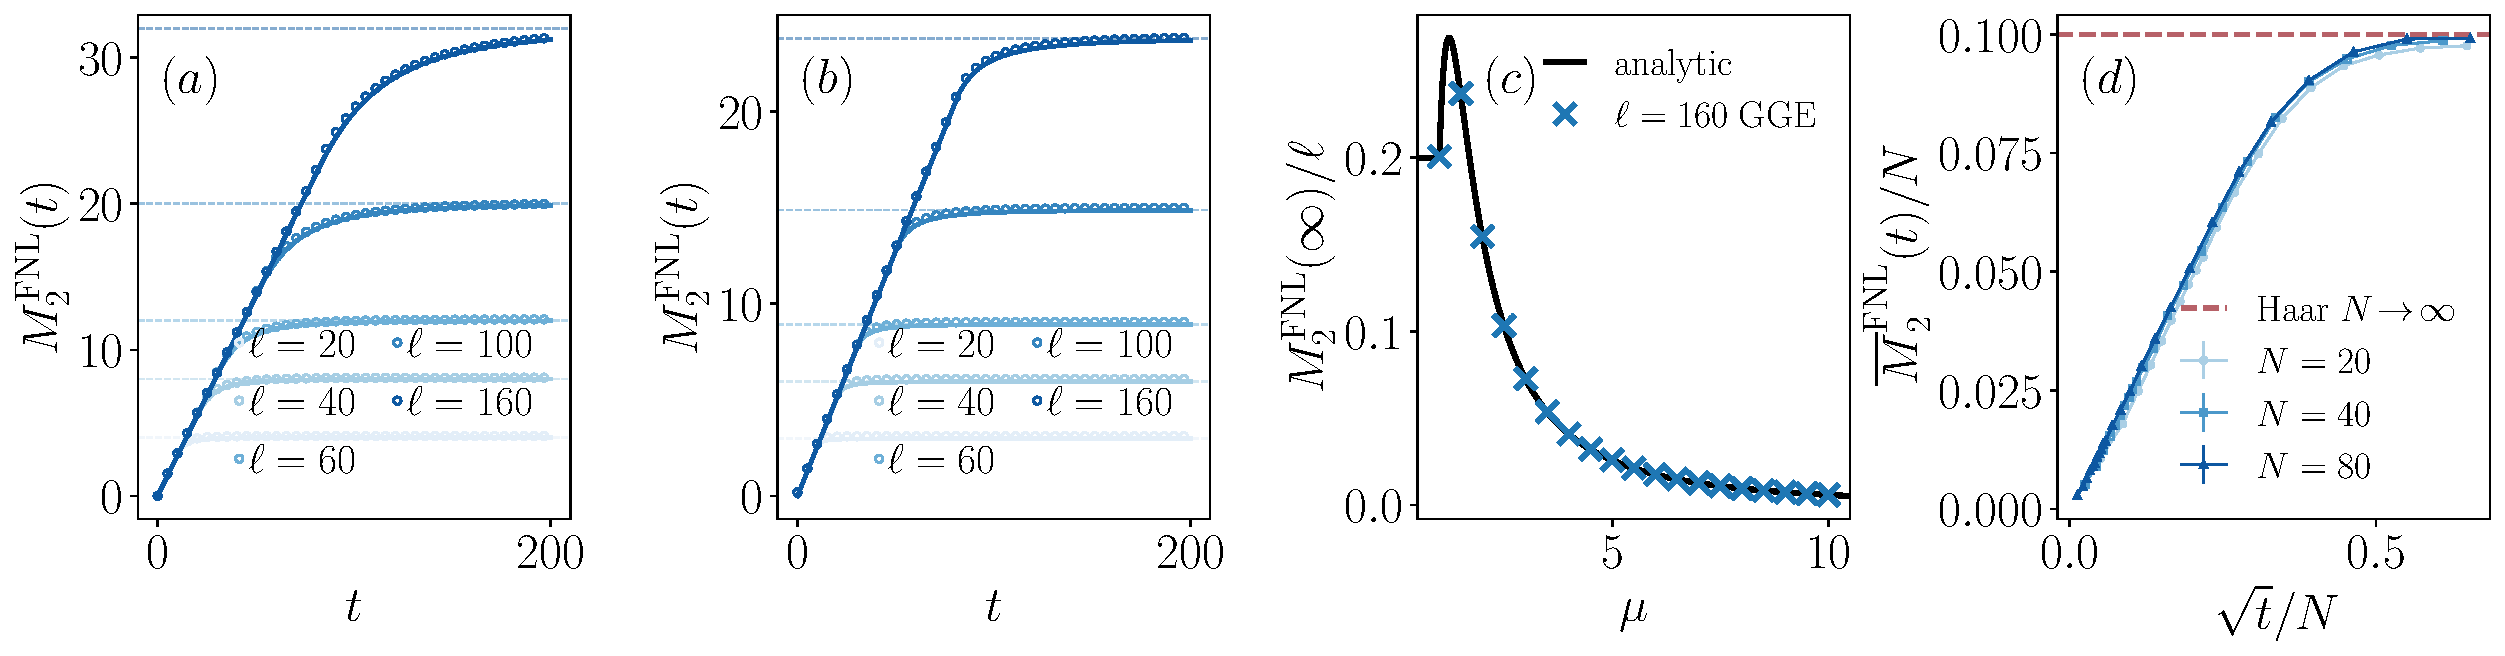
\includegraphics[width=\linewidth]{../fig2_dynamics_4panel.pdf}
    \caption{%
    \textbf{Dynamics of Gaussian-restricted non-local magic.}
    (a)~Quench at $\eta=1$ from the fully polarized state ($\mu_0\to\infty$) to the critical point ($\mu=1$): the exact numerics (circles) agrees quantitatively with the analytical prediction in Eq.~\eqref{eq:fagotti_mnl} (solid lines) for subsystem sizes $\ell = 20, 40, 60, 100, 160$. Dashed lines mark the GGE stationary value.
    (b)~Same for a finite quench $\mu_0 = 2 \to \mu = 1$, showing weaker Gaussian-restricted non-local magic production due to the smaller Bogoliubov overlap $\sin^2\Delta\theta_k$.
    (c)~Stationary-state density $M_2^{\mathrm{GNL}}(\infty)/\ell$ as a function of the post-quench field $\mu$ ($\mu_0\to\infty$): analytical prediction from Eq.~\eqref{eq:mnl_stationary} (solid) and GGE numerics at $\ell = 160$ (crosses).
    (d)~Random Gaussian circuit dynamics:  $\overline{M_2}^{\mathrm{GNL}}/N$ is plotted against $\sqrt{t}/N$ for $N = 20, 40, 80$, exhibiting diffusive growth $\sim\!\sqrt{t}$ and saturation to the fermionic Gaussian Haar-random value $\overline{\mathsf{m}}_{2}^{\mathrm{GNL}}(r=1/2)=2-\log_2(2+\sqrt{3})$  (dashed line).}
    \label{fig:dynamics}
\end{figure*}

We now turn from equilibrium to the non-equilibrium dynamics of Gaussian-restricted non-local magic, focusing on quantum quenches in the Ising chain.
The system is prepared in the ground state $|\Psi_0\rangle$ of $H(\mu_0)$ and, at time $t=0$, the transverse field is suddenly quenched to $\mu \neq \mu_0$; the state then evolves unitarily as $|\Psi(t)\rangle = e^{-iH(\mu)t/2}|\Psi_0\rangle$, where, following Refs.~\cite{Calabrese2005evolution,Fagotti2008}, we measure time in units in which the evolution is generated by $H(\mu)/2$.
Since both the initial state and the time evolution preserve the Gaussian structure, $|\Psi(t)\rangle$ remains a fermionic Gaussian state at all times, fully characterized by its time-dependent covariance matrix $\Gamma(t)$.

In particular, the time-dependent block-Toeplitz symbol of $\Gamma_A(t)$ takes the form~\cite{Calabrese2005evolution}

\subsubsection{Stationary state via dephasing}

At long times $t\to\infty$, the oscillating terms $\cos (2\varepsilon_k t)$ and $\sin(2\varepsilon_k t)$ in $p(k,t)$ and $q(k,t)$ average to zero due to dephasing across modes with different group velocities~\cite{Calabrese2005evolution}.
Only the time-independent part of $p$ survives, $p(k,\infty) = e^{-i\theta_k}\cos(\Delta\theta_k)$, while $q(k,\infty) = 0$.
The resulting stationary covariance matrix is that of a generalized Gibbs ensemble (GGE)~\cite{Calabrese2005evolution,vidmar2017entanglement} and is again a block-Toeplitz matrix, now with a \emph{time-independent} symbol.
The eigenvalues $\pm\lambda_k^\infty$ of the stationary $i\Gamma_A^\infty$ are determined by the Bogoliubov angle mismatch alone, $\lambda_k^\infty=|\cos\Delta\theta_k|$, 
 and the stationary Gaussian-restricted non-local magic density is obtained via the Szeg\H{o} theorem~\cite{Calabrese2005evolution}
\begin{equation}
    M_2^{\mathrm{GNL}}(\infty) = \frac{\ell}{\pi}\int_0^\pi\! dk\; \mathfrak{m}_2\!\left(\sin^2\!\Delta\theta_k\right)\;.
    \label{eq:mnl_stationary}
\end{equation}
This result reveals that for any $\mu\neq \mu_0$, the quench generically produces extensive (volume-law) Gaussian-restricted non-local magic; the expression is symmetric under $\mu \leftrightarrow \mu_0$.

\subsubsection{Quasiparticle picture}

Inserting Eq.~\eqref{eq:moments_asymptotic} into  Eq.~\eqref{eq:circccc} and carrying out the contour integration yields the quasiparticle formula
\begin{equation}
    M_2^{\mathrm{GNL}}(\ell,t) \simeq \int_0^\pi\!\frac{dk}{\pi}\,\min\!\bigl(2|v_k|\,t,\;\ell\bigr)\;\mathfrak{m}_2\!\bigl(\sin^2(\Delta\theta_k)\bigr),
    \label{eq:fagotti_mnl}
\end{equation}
valid in the scaling limit $\ell, t \gg 1$ with $t/\ell$ arbitrary.
Eq.~\eqref{eq:fagotti_mnl} predicts linear growth $\MNL \propto t$ for $t < t^* = \ell/(2v_{\max})$ and saturation to the extensive value $\MNL(\infty)/\ell = \pi^{-1}\int_0^\pi \mathfrak{m}_2(\sin^2\!\Delta\theta_k)\, dk$ for $t \gg t^*$.
Eq.~\eqref{eq:fagotti_mnl} has a transparent physical interpretation in terms of the quasiparticle picture~\cite{Calabrese2005evolution,Fagotti2008}: the quench creates pairs of entangled quasiparticles at each point, which propagate ballistically with mode-dependent velocities $\pm v_k$.
A pair at momentum $k$ contributes to $M_2^{\mathrm{GNL}}$ of the block $A$ only when one partner has entered $A$ while the other remains outside, hence the $\min(2|v_k|t,\ell)$ factor.
The weight $\mathfrak{m}_2(\sin^2\Delta\theta_k)$  quantifies the Gaussian-restricted non-local magic carried by each entangled pair: it vanishes both when $\Delta\theta_k = 0$ (no quench, no entanglement production) and when $\Delta\theta_k = \pi/2$ (maximally entangled but stabilizer-like mode), and is maximal at intermediate values.

We benchmark Eq.~\eqref{eq:fagotti_mnl} at $\eta=1$ (Ising chain) by  evaluating numerically Eq.~\eqref{eq:mustang}. 
Our results are reported in Fig.~\ref{fig:dynamics} for the quench $\mu_0 = \infty \to \mu = 1$ (panel (a))  and $\mu_0 = 2 \to \mu = 1$ (panel (b)) at subsystem sizes $\ell = 20, 40, 60, 100, 160$. 
The exact time evolution (markers), obtained by constructing the full block-Toeplitz $\Gamma_A(t)$ via Eq.~\eqref{eq:pq_symbol} and diagonalizing, is in excellent agreement with the semiclassical prediction (solid lines) from Eq.~\eqref{eq:fagotti_mnl}.
The dashed horizontal lines indicate the stationary values from Eq.~\eqref{eq:mnl_stationary}, which are approached at $t \simeq t^\star$.
In Fig.~\ref{fig:dynamics}(c) we benchmark the steady state $M_2^{\mathrm{GNL}}(\infty)$ with the analytical expression Eq.~\eqref{eq:mnl_stationary} for the GGE, again in perfect agreement. 

\section{Discussion}

\subsection{Summary}

We have proved an exact, closed-form expression for the fermionic Gaussian-restricted non-local magic of Gaussian states at R\'enyi index $\RENYI=2$. A generalized expression for $\RENYI>2$ is verified numerically and shares the same qualitative features.
By reducing the minimization over Gaussian unitaries, the computation simplifies to a single eigenvalue decomposition of the reduced covariance matrix, completely bypassing the prohibitive variational minimization over the full Hilbert space. This establishes fermionic Gaussian states as a broad class of highly entangled many-body systems where the related non-local magic is exactly tractable, providing a useful proxy for the non-local magic over the full Unitary group.
Beyond the physical result, the proof introduces two ingredients that we expect to be of independent interest: a sharp bound controlling the collision probability of a single Slater determinant by its transpose overlap; and a Hadamard-type determinant inequality for positive matrices of rank at most two, proved using fermionic creation operators.


We applied this framework across three key physical settings.
For typical fermionic Gaussian states, we derived an exact Page-like curve via random matrix theory, a prediction independently confirmed by SYK$_2$ mid-spectrum eigenstates.
At equilibrium, we characterized the Gaussian-restricted non-local magic of the XY spin chain ground state, obtaining exact results in both gapped and critical phases: a finite saturation value off criticality via corner transfer matrices, and logarithmic scaling at the critical point via the Fisher--Hartwig formula.
Out of equilibrium, we established a quasiparticle picture for the spreading of Gaussian-restricted non-local magic after quantum quenches, finding linear growth up to a crossing time $t^\star= \ell/(2v_\mathrm{max})$  followed by saturation to a volume-law value.
In contrast, random Gaussian circuits exhibit diffusive growth, with non-local magic scaling as $\sqrt{t}$ before saturating at the Haar-random value on a timescale $t\sim N^2$.
\clearpage
\section*{End Matter}

\subsection{Experimental observability}

A key practical advantage of Eq.~\eqref{eq:analytic_NL} is that the Gaussian-restricted non-local magic of Gaussian states is entirely determined by the reduced covariance matrix $\Gamma_A$, a polynomial number of two-point correlation functions.
While a proof-of-principle demonstration of non-local magic has recently been reported on a superconducting processor in a two-qubit setting~\cite{ahmad2025experimentaldemonstrationnonlocalmagic}, our result opens a scalable route applicable to large fermionic Gaussian systems.

A natural experimental protocol is \emph{fermionic shadow tomography}~\cite{Wan_2023}: random matchgate circuits are applied, followed by computational-basis measurements, and $\Gamma_A$ is inferred from the resulting classical-shadow data.
A conservative sample-complexity estimate yields, for failure probability at most $\delta$,
\[
N_{\mathrm{shots}} = O\!\left(\frac{\ell^2 \log(\ell/\delta)}{\epsilon_\Gamma^2}\right),
\]
to reconstruct \(\Gamma_A\) with accuracy \(\epsilon_\Gamma\), while the propagation of this error  to \(M_2^{\mathrm{GNL}}\) is discussed in  Appendix~\ref{app:experimental}.

For a fixed subsystem $A$ of size $\ell\le N/2$, let us define the stochastic variables $x_k:=\lambda_k^2$, whose joint probability distribution is a Jacobi ensemble~\cite{Mehta2004,PhysRevB.103.L241118}
\begin{equation}
    \mathbb{P}(x_1,\dots,x_\ell) = \frac{\Delta(x_1,\dots,x_\ell)}{Z_\ell}  \prod_{m=1}^\ell \frac{(1-x_m)^{N-2\ell}}{\sqrt{x_m}}\;,
\end{equation}
with $\Delta(x_1,\dots,x_\ell)=\prod_{1\le i<j\le \ell} (x_i-x_j)^2$ the squared Vandermonde determinant  and $Z_\ell$ the normalization ensuring $\int \mathbb{P}(x_1,\dots,x_\ell)\prod_{m=1}^\ell (dx_m)=1$. 
Since $M_2^\mathrm{GNL}=\sum_{m=1}^\ell \mathfrak{m}_2(x_m)$ is a sum over separate $x_m$ contributions, the only ingredient required is the one-point density function 
\begin{equation}
\begin{split}
    \varrho^{(\ell)}(x):&=\mathbb{E}_\mathbb{P}\left[\sum_{m=1}^\ell \delta(x-x_m)\right] \\&= \ell \int \mathbb{P}(x,x_2,\dots,x_\ell)\prod_{m=2}^\ell (dx_m)\:,
\end{split}
\end{equation}
where we used relabelling in the second step. Notice that $\int_0^1 \varrho^{(\ell)}(x) dx = \ell$.
Thus, the average Gaussian-restricted non-local magic is 
\begin{equation}
    \overline{M}_2^\mathrm{GNL}=\int_0^1 \mathfrak{m}_2(x) \varrho^{(\ell)}(x) dx\;.
\end{equation}
For the Jacobi ensemble, the one-point density is given by the standard orthogonal-polynomial kernel.
Given $w(x) = (1-x)^{N-2\ell}/\sqrt{x}$, we have~\cite{sierant2026theorymatchgatecommutant,sierant2026fermionic}
\begin{equation}
\varrho^{(\ell)}(x) = w(x) \sum_{n=0}^{\ell-1} [p_n(x)]^2\;,
\label{eq:ziopino}
\end{equation}
where $p_n$ are polynomials in the domain $[0,1]$, that are orthonormal with respect to the weight $w(x)$, namely $p_n(x) = \mathrm{P}_n^{(-1/2,N-2\ell)}(1-2x)/\sqrt{h_n}$ in terms of the Jacobi polynomials $\mathrm{P}_n^{(a,b)}$ and with normalization 
\begin{equation}
    h_n=\frac{\Gamma(n+1/2) \Gamma(n+N-2\ell+1)}{(2n+N-2\ell+1/2) \Gamma(n+1)\Gamma(n+N-2\ell+1/2)}.
\end{equation} 

Eq.~\eqref{eq:ziopino} yields the exact average non-local magic at finite size $N$ for a given $\ell$, which we benchmarked against direct sampling of Haar-random $O\in\mathrm{O}(2N)$, including the data of Fig.~\ref{fig:typicality}(a), finding agreement within statistical errors; the figure compares these data with the thermodynamic limit derived below.

In this regime, the rescaled  one-point density $\varrho^{(\ell)}/N$ converges to the free Jacobi law with support $x\in [0,c]$, $c=4r(1-r)$,
\begin{equation}
    \varrho_r(x) = \frac{\sqrt{(c-x)x}}{2\pi x(1-x)}\mathbf{1}_{[0,c]}(x)\;,
\end{equation}
where $\mathbf{1}_A(x)$ is the characteristic function of $A$, $\mathbf{1}_A(x)=1$ if and only if $x\in A$. 
The total mass of the density is $\int_0^c \varrho_r(x) dx=r$, which is precisely the fraction of the number of eigenvalues over the system size. 
Thus, in the scaling limit, we have
\begin{equation}
\overline{\mathsf{m}}_2^\mathrm{GNL}(r)\simeq \int_0^c \mathfrak{m}_2(x) \varrho_r(x)dx\;.
\end{equation}
A more convenient parametrization is obtained by setting $x=c\sin^2\theta$  with $\theta\in[0,\pi/2]$. Then the integral is 

Notably, for $\mu<1$ the non-local magic is strongly suppressed, $M_2^{\mathrm{GNL}}$ being exponentially small in the level spacing $\varepsilon$ of the entanglement spectrum and vanishing exactly only in the GHZ limit $\mu\to0$. This is the ordered (ferromagnetic) phase, whose ground state approaches the GHZ state $\frac{1}{\sqrt{2}}(|{+}\rangle^{\otimes N}+|{-}\rangle^{\otimes N})$, with $X|{\pm}\rangle=\pm|{\pm}\rangle$, as $\mu\to 0$. The suppression of non-local magic in this regime can be understood from the Peschel entanglement spectrum, Eq.~\eqref{eq:peschel_spectrum}: for $\mu<1$ and $\eta=1$, the single-particle entanglement energies are $\varepsilon_n^{\mathrm{ent}}=2n\varepsilon$. The $n=0$ mode has $\varepsilon_0=0$, yielding $\lambda_0=\tanh(0)=0$ (a maximally entangled, stabilizer-like Bell pair), while all $n\ge 1$ modes have $\lambda_n=\tanh(n\varepsilon)$ exponentially close to $1$ (nearly unentangled modes). Since $\mathfrak{m}_2(0)=\mathfrak{m}_2(1)=0$, every mode contributes an exponentially small amount of non-local magic. This is a striking example of a phase with nonzero entanglement entropy (area law) but negligible  non-local magic. In contrast, the entanglement entropy receives a finite area-law contribution from the $n=0$ maximally entangled mode.

We present the argument for arbitrary $\RENYI\ge1$; it is rigorous at $\RENYI=2$ by Theorem~\ref{thm:global}, while for $\RENYI\neq2$ it inherits the status of the conjectured weights of Eq.~\eqref{eq:analytic_NL_alpha}.

Let $|\Psi_O\rangle$ be such a Gaussian ground state and let $A=\{1,\dots,\ell\}$ be a contiguous block, as in Theorem~\ref{thm:global}. The Gaussian entanglement entropy is
\begin{equation}
    S(A)=
    \sum_{i=1}^{\ell}
    \mathfrak{f}\!\left(\frac{1+\lambda_i}{2}\right),
    \label{eq:gaussian_entropy_area_law_sec}
\end{equation}
where $\mathfrak{f}(x):=-x\log_2x-(1-x)\log_2(1-x)$. On the other hand, taking the limit \(\RENYI\to1\) in Eq.~\eqref{eq:analytic_NL_weights} gives
\begin{equation}
    M_{1}^{\mathrm{GNL}}(|\Psi_O\rangle)
    =
    \frac{1}{2}
    \sum_{i=1}^{\ell}
    \mathfrak{f}(\lambda_i^2).
    \label{eq:M1_GNL}
\end{equation}
Moreover, $M_{\alpha}^{\mathrm{GNL}}\le M_{\beta}^{\mathrm{GNL}}$ for $\alpha\ge\beta$, since R\'enyi entropies are non-increasing in the index. By noticing that for every $\lambda\in[0,1)$
\begin{equation}
    \frac{1}{2}\mathfrak{f}(\lambda^2)
    \le
    2\, \mathfrak{f}\!\left(\frac{1+\lambda}{2}\right),
    \label{eq:m1_entropy_bound}
\end{equation}
then, summing over the single-particle entanglement modes gives
\begin{equation}
    M_{\RENYI}^{\mathrm{GNL}}(|\Psi_O\rangle)
    \le
    M_{1}^{\mathrm{GNL}}(|\Psi_O\rangle)
    \le
    2\, S(A),
    \qquad
    \RENYI\ge1.
    \label{eq:GNL_bound_by_entropy_all_alpha}
\end{equation}
This is the Gaussian analogue of the general entanglement-controlled bound discussed for $M_2^{\mathrm{NL}}$ in Ref.~\cite{Cao_2025}.

Finally, by Hastings' theorem~\cite{Hastings_2007}, the entanglement entropy of a unique gapped ground state of a one-dimensional local Hamiltonian obeys
\begin{equation}
    S(A)\le C_{\mathrm{ent}}|\partial A|,
    \label{eq:Hastings_area_law}
\end{equation}
with $C_{\mathrm{ent}}$ independent of $|A|$ and of the total system size. Therefore
\begin{equation}
    M_{\RENYI}^{\mathrm{NL}}(|\Psi_O\rangle)
    \le
    M_{\RENYI}^{\mathrm{GNL}}(|\Psi_O\rangle)
    \le
    2\, C_{\mathrm{ent}}|\partial A|,
    \label{eq:GNL_area_law_final}
\end{equation}
whenever $\RENYI\ge1$. 

Eq.~\eqref{eq:mnl_stationary} bears a striking structural similarity to the entanglement entropy of the same quench~\cite{Calabrese2005evolution}, $S=\frac{\ell}{\pi} \int_0^\pi\! dk\; \mathfrak{f}\bigl(\sin^2(\Delta\theta_k/2)\bigr)$, with $\mathfrak{f}(x):= -(1-x)\log_2(1-x)-x\log_2(x)$  the binary entropy: in terms of the stationary eigenvalues $\lambda_k^{\infty}=|\cos\Delta\theta_k|$, the entanglement weight $\mathfrak{f}\bigl((1+\lambda_k^{\infty})/2\bigr)$ is replaced by the magic weight $\mathfrak{m}_2\bigl((\lambda_k^{\infty})^2\bigr)=\mathfrak{m}_2(\sin^2\!\Delta\theta_k)$, using the symmetry $\mathfrak{m}_2(x)=\mathfrak{m}_2(1-x)$.
This parallel extends beyond the stationary state and allows us to derive, from first principles, a quasiparticle picture for the spreading of Gaussian-restricted non-local magic.

\subsection{Random Gaussian circuit dynamics}

Finally, we consider the dynamics of Gaussian-restricted non-local magic under random Gaussian circuits~\cite{tirrito2025magicphasetransitionsmonitored}.
The circuit is composed of nearest-neighbor fermionic Gaussian unitaries arranged in a brick-wall geometry on $N$ sites.
A single layer $O_{\mathrm{layer}} = O_{\mathrm{odd}}\,O_{\mathrm{even}}$ consists of an even and an odd half-step, namely $O_{\mathrm{even}} = \prod_{j=1}^{N/2} R_{2j-1,2j}$ and $O_{\mathrm{odd}} = \prod_{j=1}^{N/2-1} R_{2j,2j+1}$, where each $R_{j,j+1} \in \mathrm{SO}(4)$ is a random orthogonal matrix drawn independently from the Haar measure, acting on the four Majorana operators $(\gamma_{2j-1}, \gamma_{2j}, \gamma_{2j+1}, \gamma_{2j+2})$ of sites $j$ and $j+1$.
The full circuit after $t$ layers is $O(t) = \prod_{s=1}^t O_{\mathrm{layer}}^{(s)} \in \mathrm{SO}(2N)$.
The initial state is the product state $|\mathbf{0}\rangle$ (vacuum of all fermionic modes), with covariance matrix $\Gamma_0$. 

The time-evolved state remains Gaussian at all times, with covariance matrix $\Gamma(t) = O(t)\,\Gamma_0\,O(t)^T$.
The Gaussian-restricted non-local magic is therefore entirely determined by the restricted covariance matrix $\Gamma_A(t)$ and its eigenvalues $\pm\lambda_j(t)$.

In contrast to the ballistic quasiparticle spreading found in the integrable quench setting, operator spreading in local random free-fermion circuits is \emph{diffusive}~\cite{dias2021diffusiveoperatorspreadingrandom,swann}.
Since the Gaussian-restricted non-local magic is a smooth spectral functional of $\Gamma_A(t)$, it inherits this diffusive transport.
At early times the modes of $A$ are nearly unentangled; expanding the single-mode contribution for $\lambda\to1$, $\mathfrak{m}_2(\lambda^2) \simeq \frac{1-\lambda^2}{\ln 2}$, so that $M_2^{\mathrm{GNL}}(t) \simeq \frac{1}{2\ln 2}\{2\ell-\mathrm{Tr}[(i\Gamma_A(t))^2]\}=\frac{1}{2\ln 2}\|\Gamma_{AB}(t)\|_{\mathrm{HS}}^2$, with $\Gamma_{AB}$ the off-diagonal block of $\Gamma$, which is governed by the diffusive spreading of two-point correlations across the entanglement cut~\cite{dias2021diffusiveoperatorspreadingrandom}.
This argument yields
\begin{equation}
    M_2^{\mathrm{GNL}}(t) \propto \sqrt{t}\;, \qquad 1 \ll t \ll N^2\;.
\end{equation}
At late times, $M_2^{\mathrm{GNL}}$ saturates to the Haar-random fermionic Gaussian value, and the natural scaling variable is $\sqrt{t}/N$.
In Fig.~\ref{fig:dynamics}(d), we plot $\overline{M_2}^{\mathrm{GNL}}(t)/N$ versus $\sqrt{t}/N$ for $N = 20, 40, 80$, finding an excellent data collapse onto a single scaling function that interpolates between $\sqrt{t}$ growth and saturation at the Page-curve value $\overline{\mathsf{m}}_{2}^{\mathrm{GNL}}(r=1/2)=2-\log_2(2+\sqrt{3})$  (dashed line).
The saturation timescale $t\sim\mathcal{O}(N^2)$ is consistent with diffusive dynamics.
\clearpage
\section*{Moved to the Supplemental Material}

\subsection{Simple example: entanglement without non-local magic}

Before presenting applications, we illustrate the physical content of the non-local magic with a simple but instructive example that clarifies the distinction between entanglement and non-local magic.
Consider $N$ qubits with $\ell = N/2$ and the rainbow state
\begin{equation}
    |\Psi_{\mathrm{rb}}\rangle = \bigotimes_{j=1}^{\ell} \frac{1}{\sqrt{2}}\bigl(|0_j 0_{\bar\jmath}\rangle + |1_j 1_{\bar\jmath}\rangle\bigr)\;,
\end{equation}
where $\bar\jmath = N+1-j$ is the mirror site in $B=\{\ell+1,\dots,N\}$, for the bipartition $A=\{1,\dots,\ell\}$. This is a fermionic Gaussian state: it is the ground state of a free-fermion hopping Hamiltonian with suitable long-range pairing. Each pair $(j,\bar\jmath)$ forms a maximally entangled Bell pair, so every eigenvalue of $i\Gamma_A$ vanishes, $\lambda_j = 0$, and the entanglement entropy is maximal: $S = \ell$ bits, a volume law. Yet, this state is a stabilizer state: it belongs to the Clifford orbit of the computational basis. Consequently its magic, and therefore its non-local magic, vanishes identically: $M_2^{\mathrm{NL}} = 0$.

This result is transparent from our formula: $\mathfrak{m}_2(\lambda_j^2)$ vanishes both at $\lambda_j = 0$  (maximally entangled mode) and at $\lambda_j = 1$  (unentangled mode). Non-local magic requires modes at \emph{intermediate} entanglement, $0 < \lambda_j < 1$, where the bipartite correlations are neither trivial nor of the Bell-pair type.

One might attempt to introduce magic into the rainbow state by applying local unitaries, e.g.\ a non-Clifford single-qubit rotation $R(\phi)$ on site $j\in A$. This produces a state $(R(\phi)\otimes \mathbb{I})|\mathrm{Bell}\rangle_{j\bar\jmath}$ that carries nonzero total magic. However, by construction, this magic is entirely \emph{local}: it can be removed by the inverse rotation $R(-\phi)\otimes \mathbb{I}$ acting on $A$ alone, and therefore does not contribute to $M_2^{\mathrm{NL}}$. The only way to create genuine non-local magic is to entangle the two qubits of each Bell pair in a non-stabilizer fashion, for instance, by applying a joint non-Clifford \emph{Gaussian} rotation $V_{j\bar\jmath}$~\cite{huang2026dismagickerunitarygatenonstabilizerness} that acts simultaneously on sites in $A$ and $B$, so that the state remains Gaussian and Theorem~\ref{thm:global} applies. Such a rotation shifts $\lambda_j$ away from $0$ and $1$, placing it in the interior of $[0,1]$ where $\mathfrak{m}_2(\lambda_j^2) > 0$. In other words, entanglement is necessary but not sufficient for non-local magic: a state can be maximally entangled yet carry zero nonstabilizerness across the bipartition.

This model is specified by the  Hamiltonian  $H$ of the form in  Eq.~\eqref{eq:ham} with  $h$ a random antisymmetric matrix whose elements are drawn from the normal distribution $h_{m,n}\sim \mathcal{N}(0,{J^2}/{N})$ and set $J=1$. 
The single-body Hamiltonian $ih$ is Hermitian with eigenvalues in $\pm\varepsilon_k$ pairs ($k=1,\dots,N$), each pair defining an effective fermionic mode. A many-body eigenstate is specified by a filling $\mathcal{F}\subset\{1,\dots,2N\}$ of $N$ single-particle modes with eigenvectors $|v_k\rangle$, yielding the one-body density matrix $\Xi=\sum_{k\in\mathcal{F}}|v_k\rangle\langle v_k|$ and the covariance matrix $\Gamma = i(2\Xi-\mathbb{I})$. 
The ground state fills the $N$ lowest-energy modes; to probe typicality, we construct mid-spectrum eigenstates $H|E_n\rangle=E_n|E_n\rangle$  by flipping a random subset of $N/4$ to $N/2$ modes from the ground-state configuration, replacing occupied negative-energy modes with their positive-energy partners. For each of $N_{\mathrm{dis}}=1000$ disorder realizations, we compute $M_2^{\mathrm{GNL}}$ from $\Gamma$ and average over 200 excited eigenstates $|E_n\rangle$ per realization, obtaining $\overline{M}_2^{\mathrm{GNL}}=\mathbb{E}_{h}\,\mathbb{E}_{n}[M_2^{\mathrm{GNL}}(|E_n\rangle)]$.

Using the Jordan--Wigner transformation, Eq.~\eqref{eq:xy} is mapped to the quadratic Hamiltonian $H$of the form in Eq.~\eqref{eq:ham} with single-body matrix entries $h_{2m-1,2m} = 2\mu$, $h_{2m,2m+1} = 1+\eta$, $h_{2m+2,2m-1} = 1-\eta$, and all remaining elements fixed by antisymmetry~\cite{Mbeng2024}. 

We restrict to system sizes $N$ divisible by $4$, for which the ground state lies in the Neveu--Schwarz sector with antiperiodic fermionic boundary
conditions $c_{N+1}=-c_1$, i.e., $\gamma_{2N+1}=-\gamma_1$ and $\gamma_{2N+2}=-\gamma_2$~\cite{Mbeng2024}.
The allowed momenta are 
$k=k(n)= \pi(2n+1)/N$ for $n = 0,\dots, N/2-1$, 
spanning $(0,\pi)$ with $N/2$ equally spaced points; 
in the thermodynamic limit $N\to\infty$, sums over $k(n)$ 
become integrals over $[0,\pi]$.
Then, the single-body Hamiltonian $ih$ is diagonalized by a Fourier transform to momentum space followed by a $2\times 2$ Bogoliubov rotation at each wave-vector $k$~\cite{Mbeng2024}.
The Bogoliubov angle $\theta_k$ is defined through
\begin{equation}
    \cos\theta_k = \frac{\mu - \cos k}{\varepsilon_k}\;,\qquad \sin\theta_k = \frac{\eta\sin k}{\varepsilon_k}\;,
    \label{eq:bogoliubov_angle}
\end{equation}
yielding the single-particle dispersion
\begin{equation}
    \varepsilon_k = \sqrt{(\mu-\cos k)^2 + \eta^2\sin^2 k}\;.
    \label{eq:dispersion}
\end{equation}
In the diagonal basis, the Hamiltonian reads $H = i\sum_k \varepsilon_k\,\tilde\gamma_{2k-1}\tilde\gamma_{2k}$, i.e., the eigenvalues of $ih$ are $\pm2\varepsilon_k$, where $\tilde\gamma_m = \sum_n G_{mn}\gamma_n$ are the rotated Majorana operators.
The ground state is the vacuum of all Bogoliubov modes, with covariance matrix $\Gamma = G\,\Gamma_0\, G^T$.

\begin{equation}
\begin{split}
    (\Gamma_A)_{mn} &= \int_{-\pi}^{\pi}\frac{dk}{2\pi}\,e^{ik(m-n)}\,g(k)\;,
    \\
    g(k) &= \begin{pmatrix} 0 & e^{i\theta_k} \\ -e^{-i\theta_k} & 0 \end{pmatrix}.
\end{split}
\label{eq:block_toeplitz}
\end{equation}

The reduced density matrix of subsystem $A$ is a fermionic Gaussian state, and can be written as~\cite{Peschel2004}
\begin{equation}
    \rho_A = \frac{\exp[{-H_{\mathrm{ent}}}]}{Z_{\mathrm{ent}}}\;, \quad H_{\mathrm{ent}} = \frac{i}{2}\sum_{n=1}^{\ell} \varepsilon_n^{\mathrm{ent}}\,\tilde\gamma_{2n-1}\tilde\gamma_{2n}\;,
    \label{eq:rho_ent}
\end{equation}
where $H_{\mathrm{ent}}$ is the entanglement Hamiltonian, $Z_{\mathrm{ent}}=\mathrm{Tr}(\exp[{-H_{\mathrm{ent}}}])$ is the normalization and $\tilde\gamma_m$ are the Majorana operators that diagonalize $\rho_A$, and $\varepsilon_n^{\mathrm{ent}} \geq 0$ are the single-particle entanglement energies.
The covariance matrix $\Gamma_A$ and the single-particle entanglement Hamiltonian $h_{\mathrm{ent}}$ implicitly defined in Eq.~\eqref{eq:rho_ent} are related by
\begin{equation}
    i\Gamma_A = \tanh\!\left(\frac{i\,h_{\mathrm{ent}}}{2}\right),
    \label{eq:Gamma_tanh}
\end{equation}
so that the eigenvalues of $i\Gamma_A$ are $\pm\lambda_n$ with $\lambda_n = \tanh\!\left(\frac{\varepsilon_n^{\mathrm{ent}}}{2}\right)$. 
Here $\lambda_n = 1$ corresponds to a pure (unentangled) mode and $\lambda_n < 1$ to an entangled one.

where $\varepsilon = \pi K(\kappa')/K(\kappa)$ is the level spacing, $K(x)$ denotes the complete elliptic integral of the first kind, $\kappa' = \sqrt{1-\kappa^2}$, and $\kappa$ is conditioned on the phase~\cite{Peschel2009}
\begin{equation}
    \kappa = \begin{cases}
        \displaystyle\frac{\eta}{\sqrt{\eta^2 + \mu^2 - 1}} & \mu > 1 \;,\\[8pt]
        \displaystyle\frac{\sqrt{\eta^2 + \mu^2 - 1}}{\eta} & \mu < 1,\; \eta^2 + \mu^2 > 1\;,\\[8pt]
        \displaystyle\sqrt{\frac{1 - \eta^2 - \mu^2}{1 - \mu^2}} & \mu < 1,\; \eta^2 + \mu^2 < 1\;.
    \end{cases}
    \label{eq:elliptic_modulus}
\end{equation}
This leads to the exact expression for the off-critical phases
\begin{equation}
    M_2^{\mathrm{GNL},\mathbb{Z}_+} = \sum_{n=0}^{\infty} \mathfrak{m}_2\!\left[\tanh^2\left(\frac{\varepsilon_n^{\mathrm{ent}}}{2}\right)\right].
    \label{eq:NL_peschel}
\end{equation}

In particular, the time-dependent block-Toeplitz symbol of $\Gamma_A(t)$ takes the form~\cite{Calabrese2005evolution}
\begin{equation}
    (\Gamma_A)_{mn}(t) = \int_0^{2\pi}\!\frac{dk}{2\pi}\,e^{ik(m-n)}\,g(k,t)\;,\label{eq:mustang}
\end{equation}
with time-dependent symbol
\begin{equation}
    g(k,t) = \begin{pmatrix} -q(k,t) & p(k,t) \\ -p(-k,t) & q(k,t) \end{pmatrix},
    \label{eq:symbol_t}
\end{equation}
where we defined the functions
\begin{equation}
\begin{split}
    p(k,t) &= e^{-i\theta_k}\left[\cos(\Delta\theta_k) + i\sin(\Delta\theta_k)\cos (2\varepsilon_k t) \right], \\
    q(k,t) &= i\,\sin(\Delta\theta_k)\,\sin (2\varepsilon_k t)\,.
    \label{eq:pq_symbol}
\end{split}
\end{equation}
Here $\varepsilon_k $ is the post-quench dispersion, $\theta_k$ is the post-quench Bogoliubov angle, and $\Delta\theta_k = \theta_k - \theta_k^{(0)}$ is the mismatch between the post-quench and pre-quench Bogoliubov angles, with
\begin{equation}
    \cos(\Delta\theta_k) = \frac{(\mu-\cos(k))(\mu_0-\cos (k))+\sin^2 (k)}{\varepsilon_k\,\varepsilon_k^{(0)}}\,.
    \label{eq:cos_delta_theta}
\end{equation}
At $t=0$, $q(k,0) = 0$ and $p(k,0) = e^{-i\theta_k^{(0)}}$, recovering the ground-state symbol of $H(\mu_0)$.
The diagonal component, $q(k,t)$, is generated dynamically by the quench and oscillates as $\sin(2\varepsilon_k t)$.

The Gaussian-restricted non-local magic can be written as a contour integral over the characteristic polynomial $D_\ell(\lambda) = \det(\lambda \mathbb{I}_{2\ell} - i\Gamma_A)$,
\begin{equation}
    M_2^{\mathrm{GNL}} = \frac{1}{4\pi i}\oint_\mathcal{C}d\lambda\;\mathfrak{m}_2(\lambda^2)\;\frac{d}{d\lambda}\ln D_\ell(\lambda)\;,\label{eq:circccc}
\end{equation}
where $\mathcal{C}$ encircles all eigenvalues counterclockwise; the factor $1/2$ compensates the double counting of the $\pm\lambda_n$ pairs.
Expanding $\ln D_\ell(\lambda)$ in powers of $\lambda^{-1}$ expresses $M_2^{\mathrm{GNL}}$ as a series in the even moments $\mathrm{Tr}(i\Gamma_A)^{2n}$.
The $2\ell \times 2\ell$ matrix $i\Gamma_A$ has a block-Toeplitz structure inherited from the symbol $g(k,t)$.
Exploiting this structure, one can show that its $2\ell$ eigenvalues coincide with those of two Hermitian matrices $W_\pm = \mathcal{H} \pm i\mathcal{T}$, where $\mathcal{T}_{jl} = \int \frac{dk}{2\pi}\,e^{-ik(j-l)}\,q(k,t)$ is Toeplitz and $\mathcal{H}_{jl} = \int \frac{dk}{2\pi}\,e^{-ik(j+l-\ell-1)}\,p(k,t)$ is Hankel. This enables the exact time dependence of $M_2^\mathrm{GNL}(t)$ following the strategy in Ref.~\cite{Fagotti2008}. 
The moments $\mathrm{Tr}(i\Gamma_A)^{2n} = \mathrm{Tr}\,W_+^{2n} + \mathrm{Tr}\,W_-^{2n}$ are then computed by expanding the matrix products into $2n$-fold momentum integrals.
As shown in Ref.~\cite{Fagotti2008}, these integrals can be evaluated exactly in the limit $\ell \gg 1$ via a multidimensional stationary phase approximation.
This procedure leads to the asymptotic expression\begin{equation}
\begin{split}
   \!\!\! \mathrm{Tr}\,(i\Gamma_A)^{2n}&\simeq \frac{2\ell}{\pi}\int_0^\pi\!\!\!dk\Bigl[1-\bigl(1-\cos^{2n}(\Delta\theta_k)\bigr)\\
   &\qquad\qquad\qquad\times\min\!\left(1, \frac{2|v_k|t}{\ell}\right)\Bigr],
\end{split}
\label{eq:moments_asymptotic}
\end{equation}
where $v_k = d\varepsilon_k/dk$ is the group velocity.

At $t=0$ the bracket equals one and all moments take the pure-state value $2\ell$, while the term proportional to $\min(1,2|v_k|t/\ell)$ interpolates ballistically towards  the stationary (GGE) moments $\frac{2\ell}{\pi}\int_0^\pi\cos^{2n}(\Delta\theta_k)\,dk$, capturing the propagation of quasiparticle pairs.

\subsection{Outlook}

The analytical tractability established here opens several natural directions for future investigation.

\emph{Higher dimensional systems.}
While our results are formulated for contiguous bipartitions of one-dimensional chains, fermionic Gaussian states in higher dimensions $D>1$ offer a rich arena where entanglement and magic may exhibit qualitatively different behavior. In two and three dimensions, a richer structure tied to the geometry of the Fermi surface is expected, and the entanglement entropy obeys an area law with multiplicative logarithmic corrections $\mathcal{O}(\ell^{D-1}\ln\ell)$~\cite{swingle2010entanglement}. 
Investigating how the scaling rate $\beta_\mathrm{GNL}$ emerges in such systems is a natural generalization.


\emph{Conformal field theory and integrable systems.}
A key question is to determine whether $\beta_{\mathrm{GNL}}$ captures universal features of the underlying conformal field theory, much as the central charge governs the scaling of entanglement entropy~\cite{Calabrese2004entanglement}.
Responding to this question requires extending our analysis to interacting integrable Hamiltonians, where Bethe-ansatz methods provide access to the entanglement spectrum.
On the dynamical side, it remains an open question whether the quasiparticle picture that successfully describes the spreading of entanglement after a quantum quench~\cite{Alba_2017,alba2019,Kudler_Flam_2021} can be adapted to account for the growth of non-local magic in these models.

\emph{Disordered systems.}
Our formula provides a natural framework to study non-local magic in the presence of quenched disorder. 
For example, in Anderson localization models~\cite{evers,sierant2020}, we expect deeply localized eigenstates to have a trivial structure, for which the Gaussian-restricted non-local magic density $\mathfrak{m}_\RENYI(x)$ vanishes. 
Similarly, free fermionic models of strongly disordered systems~\cite{IGLOI_2005,Monthus_2018,ruggiero2022}, where rare Griffiths regions and anomalous entanglement scaling emerge, are another avenue of further study.

\emph{Topological systems.}
One and two-dimensional topological phases, such as the Kitaev chain and model~\cite{Kitaev2001chain,Kitaev_2006}, host boundary modes whose non-local magic content is expected to reflect the topological invariant.
In such systems, the interplay of non-local magic and quantum coherent errors in fermionic systems is another fascinating direction to pursue~\cite{beri,gskb-t5ql}.

\emph{Interplay with symmetry.}
When the system possesses a continuous symmetry, such as $\mathcal{U}(1)$ charge conservation, the covariance matrix acquires a block structure that could enable a symmetry-resolved decomposition of $M_2^{\mathrm{GNL}}$ into contributions from different charge sectors~\cite{Goldstein}.
This connects to the broader program of symmetry-resolved entanglement~\cite{Bianchi_2022}, coherence~\cite{aditya2026coherencedynamicsquantummanybody} and stabilizer entropies, and may reveal sector-dependent magic resources~\cite{iannotti2026nonstabilizernessu1symmetrychaotic, cepollaro2025stabilizerentropysubspaces, Esposito_2024}.
An intriguing related question is whether Gaussian-restricted non-local magic exhibits quantum Mpemba-like effects~\cite{Ares_2023,Ares_2025,aditya2025mpembaeffectsquantumcomplexity}, where symmetry-broken initial conditions lead to anomalously fast relaxation of specific magic sectors.

\emph{Monitored systems and non-Hermitian dynamics.}
Hybrid systems combining unitary evolution with local measurements give rise to measurement-induced phase transitions in entanglement~\cite{FisherRandom2023,Li_2025,oshima}.
For free-fermionic setups, the dynamics remain within the Gaussian manifold, and our formula applies at each quantum trajectory.
Whether Gaussian-restricted non-local magic exhibits its own measurement-induced transition, and how it relates to the entanglement transition, is an open question.
Similarly, non-Hermitian free fermionic Hamiltonians~\cite{Ashida_2020,kawabata2026nonhermitiandisorderedsystems} generate effective Gaussian dynamics with complex spectra.
Our framework makes amenable to analytic treatment the behavior of Gaussian-restricted non-local magic in these settings~\cite{schirooooo,gallo,granet,lapierre2025entanglementtransitionsstructuredrandom}.


\bibliography{../ref_current}
\end{document}
